%Dokumentinformationen
\newcommand{\titleinfo}{Lineare Algebra - Formelsammlung}
\newcommand{\authorinfo}{C.Gwerder, S.K\"orner, M.Ehrler, L. Leuenberger}
\newcommand{\versioninfo}{v1.0}

% standard header
%Schriftgr"osse, Layout, Papierformat, Art des Dokumentes
\documentclass[10pt,twoside,a4paper,fleqn]{article}
%Einstellungen der Seitenr"ander
\usepackage[left=1cm,right=1cm,top=1cm,bottom=1cm,includeheadfoot]{geometry}
% Sprache, Zeichensatz, packages
\usepackage[utf8]{inputenc}
\usepackage[ngerman]{babel,varioref}
\usepackage{amssymb,amsmath,fancybox,graphicx,color,lastpage,wrapfig,fancyhdr,hyperref,verbatim,tabularx, arydshln,textcomp}
\usepackage{ulem}

%pdf info
\hypersetup{pdfauthor={\authorinfo},pdftitle={\titleinfo},colorlinks=false}
%linkbordercolor=white
\author{\authorinfo}
\title{\titleinfo}

%Kopf- und Fusszeile
\pagestyle{fancy}
\fancyhf{}
%Linien oben und unten
\renewcommand{\headrulewidth}{0.5pt} 
\renewcommand{\footrulewidth}{0.5pt}

\fancyhead[L]{\titleinfo{ }\tiny{(\versioninfo)}}
%Kopfzeile rechts bzw. aussen
\fancyhead[R]{Seite \thepage { }von \pageref{LastPage}}
%Fusszeile links bzw. innen
\fancyfoot[L]{\footnotesize{\authorinfo}}
%Fusszeile rechts bzw. ausen
\fancyfoot[R]{\footnotesize{\today}} 

%%%%%%%%%%%%%%%%%%%%%%%%%%%%%%%%%%%%%%%%%%%%%%%%%%%%%%%%%%%%%%%%%%%%%%%%%%%%%%%%%%%%%%%%%%%%%%%%
% Neue Befehle und Definitionen                
%%%%%%%%%%%%%%%%%%%%%%%%%%%%%%%%%%%%%%%%%%%%%%%%%%%%%%%%%%%%%%%%%%%%%%%%%%%%%%%%%%%%%%%%%%%%%%%%
\definecolor{black}{rgb}{0,0,0}
\definecolor{red}{rgb}{1,0,0}
\definecolor{white}{rgb}{1,1,1}
\definecolor{grey}{rgb}{0.8,0.8,0.8}
\newcommand{\formelbuch}[1]{$_{\textcolor{red}{\mbox{\small{S#1}}}}$}
\newcommand{\verweis}[2]{\small{(siehe auch \ref{#1}, #2 (S. \pageref{#1}))}}
\newcommand{\vektor}[3]{\left(\begin{array}{r} #1 \\ #2 \\ #3 \\ \end{array}\right)}

\begin{document}
\setlength{\parindent}{0pt} %Kein Einrücken  bei neuem Paragraph
%%%%%%%%%%%%%%%%%%%%%%%%%%%%%%%%%%%%%%%%%%%%%%%%
% Lineare Gleichungssysteme
%%%%%%%%%%%%%%%%%%%%%%%%%%%%%%%%%%%%%%%%%%%%%%%%
\section{Lineare Gleichungssysteme}

\subsection{mehere Gleichungssysteme simultan lösen}
	Dieses Gleichungssystem hat die gleiche Koeffizientenmatrix, aber verschiedene rechte  Seiten.\\
	Vorgehen:
	\begin{itemize}
		\item Für jede Gleichung eine Spalte auf der rechten Seite
		\item Gauss durchführen
			\begin{equation*}
				\begin{bmatrix} 1 & 0 \\ 0 & 1 \end{bmatrix} =  \begin{bmatrix} a_{11} & a_{12} \\ b_{11} & b_{12} \end{bmatrix}	
			\end{equation*}
		\item Lösung der Gleichung $\Rightarrow x= a_{11}z_1 + a_{12}z_2 \qquad y= b_{11}z_1 + b_{12}z_2$
	\end{itemize}

\subsection{lineare Abhängigkeit}
	\begin{tabular}{ll}
		Koeffizienten: & $A = \left(\begin{array}{cc} 1 & 4\\ 2 & 8 \end{array}\right) \left\rbrace\begin{array}{l} l_1 = x +4y \\ l_2 = 2x + 8y \end{array}\right.$\\ \\
		Bestimmung $\lambda_i$:  &  $\lambda_1 l_1 = \lambda_1 (x + 4y) = \lambda_1 x + \lambda_1 4y$ \\
		& $\lambda_2 l_2 = \lambda_2 (2x + 8y) = \lambda_2 2x + \lambda_2 8y$
	\end{tabular} \\ \\
	
	\textbf{Def.:} Wenn $\lambda_1 l_1 + \lambda_2 l_2 = 0$, alle $\lambda_i = 0$ dann ist es linear \textbf{unabhängig}. \\ \\

	$A^T = \left(\begin{array}{cc}
		1 & 2 \\
		4 & 8
	\end{array}\right) =  0 \Rightarrow \begin{array}{|cc|c|}
		\hline1 & 2 & 0\\
		4 & 8 & 0\\
		\hline
	\end{array} \rightarrow^{Gauss} \rightarrow \begin{array}{|cc|c|}
		\hline 1 & 2 & 0\\
		0 & 0 & 0\\
		\hline
	\end{array} $ \qquad somit ist $\lambda_1 = -2\lambda_2 \rightarrow$ nicht alle $\lambda_i = 0 \Rightarrow$ lin. abhängig.\\ \\

	Falls A lin. unabhängig\\
	$ A^T = \left(\begin{array}{cc}
		3 & 2\\
		-6 & 4\\
	\end{array}\right) = 0 \Rightarrow \begin{array}{|cc|c|}
		\hline 3 & 2 & 0\\
		-6 & 4 & 0 \\
		\hline
	\end{array} \rightarrow^{Gauss} \rightarrow \begin{array}{|cc|c|}
		\hline 1 & 0 & 0\\
		0 & 1 & 0\\
		\hline
	\end{array}$  \qquad somit ist $\lambda_1 = 0, \lambda_2 = 0 \Rightarrow$ lin. unabhängig.\\

	Die Linieare Abhängigkeit kann geprüft werden, indem man bei einer Matrix den Gauss durchführt. Entsteht dabei eine \textbf{leer Zeile}
	so ist es \textbf{linear abhängig}. \\
	Sind \textbf{zwei gleiche} Zeilen- bzw. Spaltenvektoren in einer Matrix, so ist sie ebenfalls \textbf{linear abhängig}.


\subsection{Bezeichnung von Matrizen und Vektoren}
	\subsubsection{Vektoren}
		\begin{tabular}{ll}
			Zeilenvektor: & $v = \left(\begin{array}{cccc} a_1 & a_2 & \ldots & a_n \end{array}\right)$ \\
			Spaltenvektor: & $v = \left(\begin{array}{c} b_1 \\ b_2 \\ \vdots \\ b_m \end{array}\right)$ \\
			Nullvektor: & $v = \left(\begin{array}{cccc} 0 & 0 & \ldots & 0 \end{array}\right)$\\
			Einheitsvektor: & $e_1 = \left(\begin{array}{cccc} 1 & 0 & \ldots & 0 \end{array}\right) \qquad 
					e_2 = \left(\begin{array}{cccc} 0 & 1 & \ldots & 0 \end{array}\right)$
		\end{tabular}
	
	\subsubsection{Matrizen}
		\begin{tabular}{ll}
			Einheitsmatrix: & $E = \left(\begin{array}{cccc}
				1 & 0 & \ldots & 0 \\
				0 & 1 &  & \vdots \\
				\vdots &  & \ddots & 0\\
				0 & \ldots & 0 & 1 \end{array}\right)$ \\
			Inverse Matrix: & $A^{-1} \qquad \begin{array}{|c|c|} \hline A & E \\ \hline \end{array} \rightarrow^{Gauss} \rightarrow
					\begin{array}{|c|c|} \hline E & A^{-1} \\ \hline \end{array} $ \\
			Transponierte Matrix: & $A^T$ \qquad Zeilen und Spalten von A vertauschen	
		\end{tabular}

\subsection{Rang}
	Maximale Anzahl linear unabhängiger Zeilen ( = linear unabhängiger Spalten)

\subsection{Homogen, Inhomogen}
	\begin{tabular}{ll}
		$Ax = b$ inhomogen & $Ax = 0$ homogen $\rightarrow b=0$\\
	\end{tabular}

	regulär $\left\lbrace\begin{array}{l}
		\text{homogen } \rightarrow \text{ Nulllösung } x=0\\
		\text{inhomogen } \rightarrow \text{ genau \underline{eine} Lösung }\end{array}\right.$ \\
	
	singulär $\left\lbrace\begin{array}{l}
		\text{homogen } Ax=0, b_1=0, b_2=0 \rightarrow \infty-\text{viele Lösungen}\\
		\text{inhomogen } Ax = b \left\lbrace\begin{array}{l}
			b_1 \neq 0, b_2 \neq 0 \rightarrow \text{ keine Lösung}\\
			b_1 \neq 0, b_2 =0 \rightarrow \infty-\text{viele Lösungen} \end{array}\right. \end{array}\right.$ \qquad 
		$ \begin{array}{|c : c|c|}
			\hline E & * & b_1 \\
			\hdashline 0 & 0 & b_2 \\
			\hline \end{array}$ \\

	Lösungsmenge eines inhomogenen Gleichungssystems mit $\infty$-vielen Lösungen\\
	$\rightarrow^{Gauss} \begin{array}{|ccc|c|}
		\hline 1 & 0 & -5 & 1 \\
		0 & 1 & 3 & 2\\
		0 & 0 & 0 & 0\\
		\hline \end{array}$ \begin{tabular}{l}
			$x = 1 + 5z$ \\
			$y = 2 - 3z$ \\
			$z = z$ \end{tabular} $\Rightarrow$ \begin{tabular}{l}
				$\mathbb{L}=\lbrace\left(\begin{array}{c}
					1+5z\\
					2-3z\\
					z \end{array}\right)\backslash z \in \mathbb{R} \rbrace$\\
				$\mathbb{L}=\lbrace\underbrace{\left(\begin{array}{c} 1 \\ 2 \\ 0 \end{array}\right)}_{x_p}
				+ \underbrace{z\left(\begin{array}{c} 5 \\ -3 \\ 1 \end{array}\right) \backslash z \in \mathbb{R}}_{\mathbb{L}_h} \rbrace$ \\
				$\mathbb{L}=\lbrace x_p + x_h \backslash x_h \in \mathbb{L}_h\rbrace$
			\end{tabular}\\

	$\mathbb{L}_h$  ist eine Gerade, Ebene... durch den Nullpunkt.


		
%%%%%%%%%%%%%%%%%%%%%%%%%%%%%%%%%%%%%%%%%%%%%%%%
% Determinante
%%%%%%%%%%%%%%%%%%%%%%%%%%%%%%%%%%%%%%%%%%%%%%%%
\section{Determinante}

\subsection{Definition einer Determinante}
	\begin{enumerate}
		\item $det(A)$ ändert sich nicht unter der Operation $E$
		\item Wird eine Zeile von $A$ mit $\lambda$ multipliziert, wird auch $det(A)$ mit $\lambda$ multipliziert: $det(\lambda A)=\lambda^{Anzahl Zeilen/Spalten}det(A)$
		\item $det(E) = 1$
	\end{enumerate}

\subsection{Eigenschaften der Determinante}
	\begin{itemize}
		\item Hat $A$ eine Nullzeile/Nullspalte, dann ist $det(A) = 0$
		\item Hat $A$ \underline{zwei gleiche} Zeilen/Spalten, dann ist $det(A) = 0$
		\item Ist $A$ regulär $\Leftrightarrow$ $det(A) \neq 0$ \\
			Ist $A$ singulär $\Leftrightarrow$ $det(A) = 0$
		\item Vertauscht man zwei Zeilen/Spalten, dann ändert sich das Vorzeichen der Determinante.
		\item Determinante = Fläche von Parallelogramm(2D) / Volumen von Parallelepipeds(3D)
	\end{itemize}

\subsection{Entwicklungssatz}
	\begin{enumerate}
		\item Zeile/Spalte auswählen (mit möglichst vielen Nullen)
		\item 1 Element herausnehmen
		\item Zeile und Spalte des herausgenommenen Elements abdecken
		\item Element mit der Determinante der nicht abgedeckten Elemente multiplizieren
		\item Schritt 2-4 wiederholen und zum 1. Element addieren/subtrahieren ($\rightarrow$ siehe Vorzeichen Matrix)
	\end{enumerate}
	
	Vorzeichenmatrix: $\begin{array}{|c|c|c|c|}
		\hline + & - & + & - \\
		\hline - & + & - & + \\
		\hline + & - & + & - \\
		\hline - & + & - & + \\
		\hline \end{array}$ \\ \\

	Beispiel: $\left|\begin{array}{ccc}
		\color{red}a & \color{green}b & \color{blue}c \\
		d & e & f \\
		g & h & i \end{array}\right| 
	= {\color{red}a} \left|\begin{array}{cc}
		e & f \\
		h & i \end{array}\right| 
	- {\color{green}b} \left|\begin{array}{cc}
		d & f \\
		g & i \end{array}\right|
	+ {\color{blue}c} \left|\begin{array}{cc}
		d & e \\
		g & h \end{array}\right|$ \\

\subsection{Wichtige Determinanten}
	$det\left(\begin{array}{cc}
		a & b \\
		c & d \end{array}\right)
	= ad - bc \qquad \qquad
	det\left(\begin{array}{ccc}
		a & b & c \\
		d & e & f \\
		g & h & i \end{array}\right)
	= \underbrace{aei + bfg + cdh - ceg - afh - bdi}_{Sarrus'sche Formel}$

\subsection{Cramsche Regel}
	$x_1= \frac{\left|\begin{array}{cccc}
		b_1 & a_{12} & \ldots & a_{1n} \\
		\vdots & \vdots & \ddots & \vdots \\
		b_n & a_{n2} & \ldots & a_{nn} \end{array}\right|}{det(A)}; \qquad
	x_2 = \frac{\left|\begin{array}{ccccc}
		a_{11} & b_1 & a_{13} & \ldots & a_{1n}\\
		\vdots & \vdots & \vdots & \ddots & \vdots \\
		a_{n1} & b_n & a_{n3} & \ldots & a_{nn} \end{array}\right|}{det(A)}$ \\ \\
	Inverse Matrix mit Cramer (Minoren): $A^{-1} = C : c_{ik} = \frac{(-1)^{k+i} \cdot det(A_{ki})}{det(A)} \longrightarrow$ 1. Index = Zeile; 2.Index = Spalte
	
	Beispiel: \ \ 
		$A=\left(\begin{array}{rrr} 
				-1 & -3 & 0 \\
				2 & 3 & -2 \\
				2 & 1 & -3 \\
			\end{array}\right)$ \\ \ \\
			
		$A^{-1}=\underbrace{\frac{1}{1}}_{det(A)}
			\left(\begin{array}{rrr} 
				+\underbrace{\left|\begin{array}{rr} 3 & -2 \\ 1 & -3 \\ \end{array}\right|}_{det(A_{11})} &
				-\underbrace{\left|\begin{array}{rr} -3 & 0 \\ 1 & -3 \\ \end{array}\right|}_{det(A_{21})} &
				+\underbrace{\left|\begin{array}{rr} -3 & 0 \\ 3 & -2 \\ \end{array}\right|}_{det(A_{31})} \\
			
				-\underbrace{\left|\begin{array}{rr} 2 & -2 \\ 2 & -3 \\ \end{array}\right|}_{det(A_{12})} &
				+\underbrace{\left|\begin{array}{rr} -1 & 0 \\ 2 & -3 \\ \end{array}\right|}_{det(A_{22})} &
				-\underbrace{\left|\begin{array}{rr} -1 & 0 \\ 2 & -2 \\ \end{array}\right|}_{det(A_{32})} \\
			
				+\underbrace{\left|\begin{array}{rr} 2 & 3 \\ 2 & 1 \\ \end{array}\right|}_{det(A_{13})} &
				-\underbrace{\left|\begin{array}{rr} -1 & -3 \\ 2 & 1 \\ \end{array}\right|}_{det(A_{23})} &
				+\underbrace{\left|\begin{array}{rr} -1 & -3 \\ 2 & 3 \\ \end{array}\right|}_{det(A_{33})} \\
			\end{array}\right)
			=\left(\begin{array}{rrr} 
				-7 & -9 & 6 \\
				2 & 3 & -2 \\
				-4 & -5 & 3 \\
			\end{array}\right)$
			
\subsection{Spezielle Fälle}
	$det\left(\begin{array}{cc} 
			A & 0 \\
			0 & B \\
		\end{array}\right)=det(A)det(B)$ \ \ wobei $det(A)$ und $det(B)$ Matrizen von Grösse $n*n$ sind.
%%%%%%%%%%%%%%%%%%%%%%%%%%%%%%%%%%%%%%%%%%%%%%%%
% Vektorgeometrie
%%%%%%%%%%%%%%%%%%%%%%%%%%%%%%%%%%%%%%%%%%%%%%%%
\section{Vektorgeometrie}

\subsection{Gerade}
	Parametergleichung: \begin{tabular}{ll}
		& $\vec{p_0} = $ Stützvektor \\
		$g = \lbrace\vec{p_0} + t\vec{r} | t \in \mathbb{R}\rbrace$ & $\vec{r} = $ Richtungsvektor \\
		& $t = $ Paramter
	\end{tabular}

	\subsubsection{Punkt auf Geraden}
		$\vec{q} = \vec{p_0} + t\vec{r} \Longrightarrow \begin{array}{|c|c|}
			\hline r_1 & q_1 - p_{01}\\
			\hline r_2 & q_2 - p_{02}\\
			\hline \end{array} \rightarrow^{Gauss} 
		\begin{array}{|c|c|}
			\hline 1 & * \\
			\hline 0 & \color{red}*\\
			\hline \end{array}$ \qquad 
		\begin{tabular}{l}
			${\color{red}*} \neq 0 \Rightarrow$ keine Lösung\\
			${\color{red}*} = 0 \Rightarrow$ $t$ eindeutig; $t$ durch erste Gleichung ausrechnen
		\end{tabular}
	
	\subsubsection{Schnittgerade}
		Beide Geraden gleichsetzen und nach $t$ auflösen $\left\lbrace\begin{array}{l}
			\text{regulär: } t \text{ ist eindeutig}\\
			\text{singulär: } \left\lbrace\begin{array}{l}
				\infty \text{ Lösungen } \rightarrow \text{ Geraden liegen aufeinander}\\
				0 \text{ Lösungen } \rightarrow \text{ Geraden sind parallel}
			\end{array}\right.
		\end{array}\right.$


\subsection{Ebene}
	Parametergleichung: \begin{tabular}{ll}
		& $\vec{p_0} =$ Stützvektor\\
		$\tau = \lbrace\vec{p_0} + t_1\vec{r_1} + t_2\vec{r_2} | t_1, t_2 \in \mathbb{R}\rbrace$ & $\vec{r_1}, \vec{r_2} =$ Spannvektoren \\
		& $t_1, t_2 =$ Paramter
	\end{tabular}

	\subsubsection{Hessche Normalform}
		$ax + by + cz - d = 0$\\
		$\vec{n_0} \bullet (\vec{p} - d) = 0$\\
		$d = \vec{p_0} \bullet \vec{n_0} = \vec{p_0} \bullet \frac{\vec{n}}{|\vec{n}|} \qquad \qquad
		d = $ Abstand von Nullpunkt zu Ebene wenn $\left|\vektor{a}{b}{c}\right| = 1$ (Länge/Betrag)

	\subsubsection{Speziallfälle der Koordinatengleichung}
		\begin{tabular}{ll}
			$a = 0 \Rightarrow by + cz = d$ & Ebene ist parallel zur $x$-Achse (äguivalent bei b und c)\\
			$a = b = 0 \Rightarrow cz = d$ & Ebene ist parallel zur $x$ und $y$- Koordinatenebene\\
			$d = 0 \Rightarrow ax + by + cz = 0$ & Ebene enthält Ursprung 0 des Koordinatensystems
		\end{tabular}

	\subsubsection{Achsenabschnittgleichung der Ebene}
		Beispiel: $\tau = 3x + 6y + 4z = 18 \Leftrightarrow \frac{3a + 6y + 4z}{18} = 1 \Leftrightarrow \frac{3}{18}x + \frac{6}{18}y + \frac{4}{18}z = 1
		\Leftrightarrow \frac{x}{6} + \frac{y}{3} + \frac{z}{4.5} = 1$\\
		Die Achsenabschnitte der Ebene $\tau$ liegen nun bei $x = 6, y = 3, z = 4.5$.\\
		Allgemeine Achsenabschnittgleichung: $$ \frac{x}{p_x} + \frac{y}{p_y} + \frac{z}{p_z} = 1$$

\subsection{Kreis und Kugel}
	Parametergleichung: \begin{tabular}{ll}
		& $\vec{m} =$ Mittelpunkt \\
		$K(M,r) = \lbrace (\vec{p} - \vec{m}) \cdot (\vec{p} - \vec{m}) = r^2 \rbrace$ & $\vec{p} =$ Punkt am äusseren Rand\\
		& $r =$ Radius
	\end{tabular}\\

	\begin{equation*}
		(\vec{p} - \vec{m})^2 = r^2  \qquad \Leftrightarrow \qquad (p_1 - m_1)^2 + (p_2 - m_2)^2 + (p_3 - m_3)^2 = r^2
	\end{equation*}

	\subsubsection{Tangentialebene}
		\begin{tabular}{lll}
			$(\vec{p_0} - \vec{m})(\vec{p} - \vec{p_0}) = 0$ & & $\vec{p_0} =$ Berührpunkt\\
			$r \cdot (\vec{p} - \vec{p_0}) = 0$ & & $\vec{p} =$ Punkt auf der Tangente\\
			$(\vec{p_0} - \vec{m})^2 = r^2$ & & $\vec{m} =$ Mittelpunkt des Kreises/Kugel
		\end{tabular}

	\subsubsection{Schnittprobleme}
		Durch Einsetzen von $x_1:=b-x_2$ in die Kreisgleichung ergibt sich eine
		quadratische Gleichung. Eine Gerade bzw. ein Kreis
		$\left\{\begin{array}{l}\mbox{meidet}\\ \mbox{berührt}\\ \mbox{schneidet}\end{array}\right\}$ einen
		anderen Kreis, wenn diese Gleichung
		$\left\{\begin{array}{l}0\\1\\2\end{array}\right\}$ Lösungen hat. Die Gerade
		heisst dann
		$\left\{\begin{array}{l} \mbox{Passante}\\ \mbox{Tangente}\\ \mbox{Sekante}\end{array}\right\}$. 
	
		Beim Schneiden zweier Kugeln ergibt sich eine \textit{Potenzebene}, bei zwei Kreisen eine
		\textit{Potenzgerade} oder \textit{Chordale}.



\subsection{Einheitsvektor}
	Der Einheitsvektor von $\vec{a} \neq 0$ hat die gleiche Richtung wie $\vec{a}$ und den Betrag 1:
	\begin{equation*}
		\vec{a_0} = \frac{\vec{a}}{|\vec{a}|}
	\end{equation*}

\subsection{Skalarprodukt}
	$\vec{v_1} \cdot \vec{v_2} = \vektor{x_1}{y_1}{z_1} \bullet \vektor{x_2}{y_2}{z_2}= x_1\cdot x_2 + y_1\cdot y_2 + z_1\cdot z_2$
	
	\subsubsection{Algebraische Eigenschaften des Skalarproduktes}
		\begin{tabular}{ll}
			$\vec{a} \bullet \vec{b} = \vec{b} \bullet \vec{a}$ & (Kommutativgesetz)\\
			$(\lambda \cdot \vec{a}) \bullet \vec{b} = \lambda \cdot (\vec{a} \bullet \vec{b}) = \vec{a} \bullet (\lambda \cdot \vec{b})$ & (gemischtes Assoziativgesetz)\\
			$(\vec{a} + \vec{b}) \bullet \vec{c} = \vec{a} \bullet \vec{c} + \vec{b} \bullet \vec{c}$ & (Distributivgesetz)
		\end{tabular}


	\subsubsection{Eigenschafen des Skalarproduktes}
		\begin{enumerate}
			\item Länge: $\vec{a} \bullet \vec{a} = |\vec{a}|\cdot |\vec{a}| \cdot \cos0 = |\vec{a}|^2$
			\item Winkel zwischen zwei Vektoren: $\vec{a} \bullet \vec{v} = \sqrt{\vec{a}\cdot \vec{a}} \cdot \sqrt{\vec{v} \cdot \vec{v}} \cdot \cos\alpha$\\
				\begin{equation*}
					\cos\alpha = \frac{\vec{a}\bullet \vec{v}}{|\vec{a}| \cdot |\vec{v}|} = \frac{\vec{a}\bullet \vec{v}}{\sqrt{\vec{a}^2} \cdot \sqrt{\vec{v}^2}}
				\end{equation*}
			\item Orthogonalität: \\
				\begin{minipage}{6cm}
					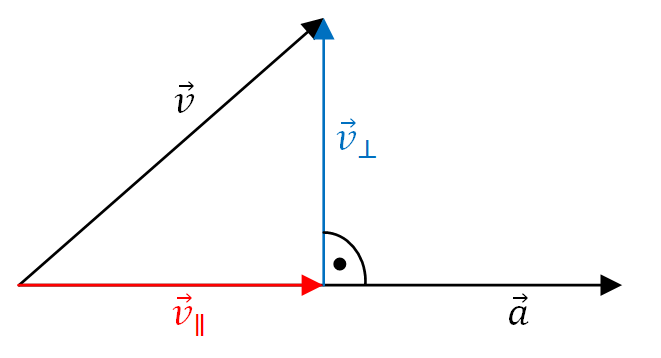
\includegraphics[width=6cm]{pics/1_Projektion.png}
				\end{minipage}
				\begin{minipage}[c]{8cm}
					\begin{equation*} P\vec{a}(\vec{v}) = |\vec{v}|\cdot \cos\alpha = \frac{\vec{a}\bullet \vec{v}}{|\vec{a}|}\end{equation*}
					\begin{equation*} v_{\parallel} = \frac{\vec{a}\bullet \vec{v}}{\vec{a}\cdot \vec{a}}\cdot \vec{a}\end{equation*}
					\begin{equation*} v_{\perp} = \vec{v} - \frac{\vec{a}\bullet \vec{v}}{\vec{a}\cdot \vec{a}}\cdot \vec{a}\end{equation*}
				\end{minipage}
		\end{enumerate}

	\subsubsection{Normalengleichung}
		\begin{equation*}
			\vec{n} \cdot (\vec{a} - \vec{p}) = 0
		\end{equation*}
		Der Normalenvektor $\vec{n}$ steht senkrecht zur Geraden oder zur Ebene. Mit seiner Hilfe und einem Punkt P ($\vec{0P} = \vec{p}$) lässt sich
		die Koordinatengleichung direkt hinschreiben:
		\begin{equation*}
			n_1 + n_2y + n_3z = \vec{n_0} \cdot \vec{p}
		\end{equation*}
		Umgekehrt lässt sich aus der Koordinatengleichung die Normalengleichung herauslesen. \\

		\textbf{Beispiel 1:} Gegebene Punkte: $A=\vektor{2}{2}{-2}$
									 $B=\vektor{3}{-3}{-1})$ \\ \ \\
							 Normale kann mithilfe des Vektorproduktes gefunden werden: \\ \ \\
									 $\vektor{n_1}{n_1}{n_1}\bullet\vektor{2}{2}{-2}=2n_1+2n_2-2n_3$ und
									 $\vektor{n_1}{n_1}{n_1}\bullet\vektor{3}{-3}{-1}=3n_1-3n_2-n_3$\\ \ \\ \ \\
							$\begin{array}{|rrr|r|}
								\hline 
									2 & 2 & -2 & 0 \\
									3 & -3 & -1 & 0 \\
								\hline
							\end{array}$
							$\rightarrow^{...}\rightarrow$	
							$\begin{array}{|rrr|r|}
								\hline 
									1 & 0 & \frac{-2}{3} & 0 \\
									0 & 1 & \frac{-1}{3} & 0 \\
								\hline
							\end{array}$
							$\rightarrow$
							$\vec{n}=\vektor{2}{1}{3}$ für $n_3 = 3$ ($n_3$ ist frei wählbar)\\
	 \textbf{Beispiel 2:} $3x-2y-z=-4\rightarrow\vec{n}=\vektor{3}{-2}{-1}$
		
\subsection{Verhalten zweier Objekte}
	\subsubsection{Schnittwinkel}
		Es wird der spitze Winkel zwischen \ldots{ }berechnet (g, h sind Geraden; E, F Ebenen; m und n Normalen):\\
		\begin{tabular}{llll}
		g $\wedge$ h:
		&$g: \vec{x}=\vec{p}+r\vec{v}$ 
		&$h: \vec{x}=\vec{q}+s\vec{w}$ 
		&$\alpha=\arccos{\frac{|v\bullet w|}{|\vec{v}|\cdot|\vec{w}|}}$\\
		g $\wedge$ h:
		&$g: m_1x+m_2y=b$
		&$h: n_1x+n_2y=c$
		&$\alpha=\arccos{\frac{|m\bullet n|}{|\vec{m}|\cdot|\vec{n}|}}$\\
		g $\wedge$ E:
		&$g: \vec{x}=\vec{p}+r\vec{v}$
		&$E: n_1x+n_2y+n_3z=b$
		&$\alpha=\arcsin{\frac{|v\bullet n|}{|\vec{v}|\cdot|\vec{n}|}}$\\
		E $\wedge$ F:
		&$E: m_1x+m_2y+m_3z=b$
		&$F: n_1x+n_2y+n_3z=c$
		&$\alpha=\arccos{\frac{|m\bullet n|}{|\vec{m}|\cdot|\vec{n}|}}$\\
		\end{tabular}

	\subsubsection{Gegenseitige Lage}
		Es werden jeweils zwei Objekte gleichgesetzt (g, h sind Geraden; E, F
		Ebenen).\\
		\begin{tabular}{lllll}
			&&$g = h$ &$g = E$ &$E = F$\\
			Keine Lösung &$\Rightarrow$ &kollinear oder windschief &parallel
			&parallel\\
			1 Lösung &$\Rightarrow$ &1 Schnittpunkt &1 Schnittpunkt & - \\
			$\infty$ Lösungen (1 Parameter frei wählbar) &$\Rightarrow$ 
			&g und h sind identisch &g liegt in E &1 Schnittgerade ($\vec{n}_E \times \vec{n}_F$) \\
			$\infty$ Lösungen (2 Parameter frei wählbar) &$\Rightarrow$  
			& - & - &E und F sind identisch
		\end{tabular}


\subsection{Orthonormalisierung}
	$\vec{a_1}, \vec{a_2}, \vec{a_3}$ sind linear unabhängig $\longrightarrow \vec{b_1} \bot \vec{b_2} \bot \vec{b_3}$\\
	\begin{minipage}{3cm}
		\begin{equation*}
			\vec{b_1} = \frac{\vec{a_1}}{|\vec{a_1}|}
		\end{equation*}
	\end{minipage}
	\begin{minipage}{5cm}
		\begin{equation*}
			\vec{b_2} = \frac{\vec{a_2} - (\vec{a_2} \bullet \vec{b_1}) \vec{b_1}}{|\vec{a_2} - (\vec{a_2} \bullet \vec{b_1}) \vec{b_1}|}
		\end{equation*}
	\end{minipage}
	\begin{minipage}{5cm}
		\begin{equation*}
			\vec{b_3} = \frac{\vec{a_3} - (\vec{a_3} \bullet \vec{b_1})\vec{b_1} - (\vec{a_3} \bullet \vec{b_2})\vec{b_2}}
					{|\vec{a_3} - (\vec{a_3} \bullet \vec{b_1})\vec{b_1} - (\vec{a_3} \bullet \vec{b_2})\vec{b_2}|}
		\end{equation*}
	\end{minipage} \\ \ \\
	
	\textbf{Beispiel:} $\vec{a_1}=\vektor{1}{0}{0}
						\vec{a_2}=\vektor{1}{1}{0}
						\vec{a_3}=\vektor{1}{1}{1}$ \\
						
						$\vec{b_1}=\frac{\vektor{1}{0}{0}}{\left|\vektor{1}{0}{0}\right|}=\vektor{1}{0}{0}$ \\
						$\vec{b_2}=\frac{\vektor{1}{1}{0}-\left(\vektor{1}{1}{0}\bullet\vektor{1}{0}{0}\right)\vektor{1}{0}{0}}{\left|\vektor{1}{1}{0}-\left(\vektor{1}{1}{0}\bullet\vektor{1}{0}{0}\right)\vektor{1}{0}{0}\right|}=\vektor{1}{1}{0}$\\
						$\vec{b_3}=\frac{\vektor{1}{1}{1}-\left(\vektor{1}{1}{1}\bullet\vektor{1}{0}{0}\right)\vektor{1}{0}{0}-\left(\vektor{1}{1}{1}\bullet\vektor{1}{1}{0}\right)\vektor{1}{1}{0}}{\left|\vektor{1}{1}{1}-\left(\vektor{1}{1}{1}\bullet\vektor{1}{0}{0}\right)\vektor{1}{0}{0}-\left(\vektor{1}{1}{1}\bullet\vektor{1}{1}{0}\right)\vektor{1}{1}{0}\right|}=\vektor{0}{0}{1}$

\subsection{Mittelsenkrechte}
	\begin{equation*}
		\vec{M_{AB}} = \frac{\vec{a} + \vec{b}}{2}
	\end{equation*}

\subsection{Least Squares}
	$A^tAv = A^tb \longrightarrow$ nach $v$ auflösen und den kleinsten Abstand zu bekommen. \qquad $(Av = b)$
		
\subsection{Vektorprodukt/Kreuzprodukt}
	\begin{equation*}
		\vec{c} = \vec{a} \times \vec{b} = \vektor{a_1}{a_2}{a_3} \times \vektor{b_1}{b_2}{b_3} = \left(\begin{array}{c}
			a_2b_3 - a_3b_2\\
			a_3b_1 - a_1b_3\\
			a_1b_2 - a_2b_1
		\end{array}\right)
		=\left(\begin{array}{c}
			\left|\begin{array}{cc}
				a_2 & b_2 \\
				a_3 & b_3 \end{array}\right|\\
			-\left|\begin{array}{cc}
				a_1 & b_1 \\
				a_3 & b_3 \end{array}\right|\\
			\left|\begin{array}{cc}
				a_1 & b_1 \\
				a_2 & b_2 \end{array}\right|
		\end{array}\right)
	\end{equation*}

	\begin{tabular}{ll}
		Zwischenwinkel: &
		\begin{equation*}
			\sin\alpha = \frac{|\vec{a} \times \vec{b}|}{|\vec{a}||\vec{b}|}
		\end{equation*}
	\end{tabular}\\ \\

	Mit Hilfe des Vektorproduktes lässt sich der \textbf{Normalenvektor}
	zweier Vektoren bestimmen. Ausserdem entspricht der Betrag des Vektorproduktes
	dem \textbf{Flächeninhalt} des von den Vektoren $\vec{a}$ und $\vec{b}$
	aufgespannten Parallelogramms. Somit sind $\vec{a}$ und $\vec{b}$ also
	kollinear, wenn $\vec{a}\times\vec{b}=0$. Das Vektorprodukt ist ein
	\textbf{Rechtssystem}
	($\vec{a} \Leftrightarrow$ Daumen; $\vec{b} \Leftrightarrow$ Zeigefinger;
	$\vec{c} \Leftrightarrow$ Mittelfinger). Das Vektorprodukt gilt nur in 3D (im
	Falle eines 2 dimensionalen Systems gilt einfach $a_3 = b_3 = 0$).

	\subsubsection{Algebraische Eigenschaften des Vektorproduktes}
		\begin{tabular}{ll}
			$\vec{a}\times\vec{b} = -(\vec{b}\times\vec{a}) = -\vec{b}\times\vec{a}$
			&(Anti-Kommutativgesetz)\\
			$(r\cdot\vec{a})\times\vec{b} = r(\vec{a}\times\vec{b}) = \vec{a}\times(r\cdot\vec{b})$
			&(gemischtes Assoziationsgesetz)\\
			$(\vec{a}+\vec{b})\times\vec{c} = (\vec{a}\times\vec{c})+(\vec{b}\times\vec{c})
			= \vec{a}\times\vec{c}+\vec{b}\times\vec{c}$\\
			$\vec{a}\times(\vec{b}+\vec{c}) = (\vec{a}\times\vec{b})+(\vec{a}\times\vec{c})
			= \vec{a}\times\vec{b}+\vec{a}\times\vec{c}$ &(Distributivgesetz)
		\end{tabular}
	
	\subsubsection{Volumen eines Parallelpipeds}
		\begin{equation*}
			det(A) = |\vec{a}; \vec{b}; \vec{c}| = (\vec{a} \times \vec{b}) \bullet \vec{c} = a_1b_2c_3 + a_2b_3c_1 + a_3b_1c_2 - c_1b_2a_3 - c_2b_3a_1 - c_3b_1a_2
		\end{equation*}

		$|\vec{a}; \vec{b}; \vec{c}| = 0 \Leftrightarrow \vec{a}; \vec{b}; \vec{c}$ komplanar \qquad 
		$|\vec{a}; \vec{b}; \vec{c}| > 0 \Leftrightarrow \vec{a}; \vec{b}; \vec{c}$ bilden Rechtssystem \qquad
		$|\vec{a}; \vec{b}; \vec{c}| < 0 \Leftrightarrow \vec{a}; \vec{b}; \vec{c}$ bilden Linkssystem

	\subsubsection{Anwendung}
		Abstand Punkt/Ebene, Gerade/Gerade:
		\begin{equation*}
			d = (\vec{p_1} - \vec{p_2}) \cdot \vec{n_0} = (\vec{p_1} - \vec{p_2}) \cdot \frac{\vec{r_1} \times \vec{r_2}}{|\vec{r_1} \times \vec{r_2}|}
		\end{equation*} 

		Abstand Punkt/Gerade:
		\begin{equation*}
			d = \frac{\vec{r} \times (\vec{p} - \vec{p_0})}{|\vec{r}|}
		\end{equation*}




























%%%%%%%%%%%%%%%%%%%%%%%%%%%%%%%%%%%%%%%%%%%%%%%%
% Vektorräume
%%%%%%%%%%%%%%%%%%%%%%%%%%%%%%%%%%%%%%%%%%%%%%%%
\newpage
\section{Vektorräume}

\subsection{Rechenregeln und Definition}
	\begin{tabular}{| l | l |}
		\hline v0: & $a + b = b + a$\\
			& $a + (b + c) = (a + b) + c$\\
		\hline v1: & $0 \in \mathbb{R}, 0 = (0, \ldots, 0) \qquad v + 0 = v \qquad \forall v$\\
		\hline v2: & zu $v \in \mathbb{R}^n$ gibt es ein $-v = (-v_1, \ldots, -v_n)$ \qquad mit $v + (-v) = 0$\\
		\hline v3: & $0 \cdot v = 0 \qquad 1 \cdot v = v$\\
		\hline v4: & $\lambda(u + v) = \lambda u + \lambda v$\\
			& $(\lambda + \mu) \cdot u = \lambda u + \mu u$\\
			& $(\lambda\mu)u = \lambda(\mu u)$\\
		\hline
	\end{tabular}\\ \\

	\textbf{Def.:} Eine Menge $V$ mit den Rechenregeln v0-v4 heisst Vektorraum, $v \in V$ heissen Vektoren.

\subsection{lineare Approximation}
	\begin{equation*}
		\left(\begin{array}{c}
			a_0 + a_1x_0 + a_2{x_0}^2 + \ldots + a_n{x_0}^n\\
			a_0 + a_1x_1 + a_2{x_1}^2 + \ldots + a_n{x_1}^n\\
			\vdots \\
			a_0 + a_1x_n + a_2{x_n}^2 + \ldots + a_n{x_n}^n\\
		\end{array}\right) = \left(\begin{array}{c}
			f(x_0)\\
			f(x_1)\\
			\vdots\\
			f(x_n)
		\end{array}\right) \Rightarrow \left(\begin{array}{ccccc}
			1 & x_0 & {x_0}^2 & \ldots & {x_0}^n\\
			1 & x_1 & {x_1}^2 & \ldots & {x_1}^n\\
			\vdots & \vdots & & \vdots \\
			1 & x_n & {x_n}^2 & \ldots & {x_n}^n\\
		\end{array}\right) \cdot \left(\begin{array}{c}
			a_0\\
			a_1\\
			\vdots \\
			a_n
		\end{array}\right) = \left(\begin{array}{c}
			f(x_0)\\
			f(x_1)\\
			\vdots \\
			f(x_n)
		\end{array}\right)
	\end{equation*}

\subsection{Spur}
	Die Spur ist die Summe der Diagonalelemente einer Matrix $Spur(A) = \Sigma a_{ii}$\\
	$Spur(ABC) = Spur(CAB) = Spur(BCA) \rightarrow$ zyklisch vertauschbar


\subsection{Basis}
	\textbf{Def.:} Sei also $V$ ein Vektorraum. Eine Menge $B = \lbrace b_1, b_2, \ldots \rbrace$ linear unabhängiger Vektoren
	ist eine Basis, wenn jeder Vektor von $V$ als Linearkombination von Vektoren aus $B$ dargestellt werden kann. Ein 
	Vektorraum heisst endlichdimensional, wenn er eine endliche Basis hat. 

\subsection{Basistransformation}
	\begin{minipage}{7cm}
		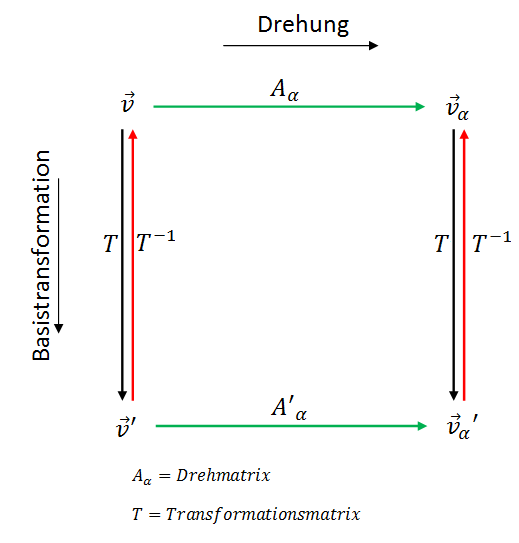
\includegraphics[width=7cm]{pics/2_Basistransformation.png}
	\end{minipage}
	\begin{minipage}{7cm}
		\begin{tabular}{ll}
			& $A =$ Matrix in alter Basis\\
			$A' = TAT^{-1}$ & $A' =$ Matrix in neuer Basis\\
			& $T =$ Transformationsmatrix\\
			$\xi' = T\xi$& $\xi =$ Vektor in der alten Basis\\
			& $\xi' =$ Vektor in der neuen Basis
		\end{tabular}
	\end{minipage}

	\subsubsection{Bestimmen der Transformationsmatrix $T$}
		$B = \underbrace{\lbrace b_j \rbrace}_{alte Basis} \qquad B' = \underbrace{\lbrace b_j' \rbrace}_{neue Basis}$\\ \\

		\textbf{Variante 1 (mit $\beta$):}\\
		Mit Gleichungssystem herausfinden, wie viele von der neuen Basis gebraucht wird um die alte darzustellen.\\
		$b_j = \beta_{j1}b_1' + \beta_{j2}b_2' + \ldots + \beta_{jn}b_n' \rightarrow$ daraus folgt $\beta$\\
		\begin{equation*}
			\mathbf{T = \beta^t}
		\end{equation*}

		\textbf{Variante 2:}\\
		Oftmals ist $b_j'$ mit den Koordinaten von der alten Basis angegeben\\
		$b_j' = \beta_{j1}b_1 + \beta_{j2}b_2 + \ldots + \beta_{jn}b_n$\\
		$\Rightarrow$ Koordinaten in der alten Basis von $b_j'$ in die Spalten der Matrix einfüllen, welches gleich $\mathbf{T^{-1}}$ ist.\\
		\begin{equation*}
			\mathbf{T = (T^{-1})^{-1}}
		\end{equation*}

	\subsubsection{Eigenschaften einer Basistransformation}
		Ein Basiswechsel ändert die Spur und die Determinante nicht!\\
		\begin{equation*}
			Spur(TAT^{-1}) = Spur(T^{-1}TA) = Spur(A)
		\end{equation*}
		\begin{equation*}
			det(TAT^{-1}) = det(T^{-1}) \cdot det(A) \cdot det(T) = det(A)
		\end{equation*}

\subsection{Lineare Abbildungen}
	\subsubsection{Orientierung}
		\begin{tabular}{lp{13cm}}
			$GL_n(\mathbb{R}) = \lbrace A | det(A) \neq 0\rbrace$ & "general linear group'' enthält alle lineare Abbildungen\\
			& $det(A)\left\lbrace\begin{array}{cc}
				>0 & \text{Rechtssystem}\\
				<0 & \text{Linkssystem}
				\end{array}\right.$ \\ \\

			$SL_n(\mathbb{R}) = \lbrace A | det(A) = 1 \rbrace$ &  ''special linear group'' enthält alle volumen- und orientierungstreue Matrizen\\
			& $det(A) =$ Volumenänderungsfaktor \\ \\

			$O(n) = \lbrace A | A^tA = E \rbrace$ & enthält alle orthogonalen Matrizen, die Längen und Winkel bleiben erhalten.\\
			& Die Detereminante ist dabei $det(A) = \pm1$ (Zeilen-/Spaltenvektoren sind orthogonal) ($OO^t = E$)
		\end{tabular}\\ \\

		\begin{tabular}{ll}
			$SO(n) = \lbrace A \in GL_n(\mathbb{R}) | det(A) = 1, A^tA = E \rbrace$ & Drehmatrizen, Volumen, Längen und Winkel bleiben 					erhalten.
		\end{tabular}

	\subsubsection{Drehwinkel}
		\begin{tabular}{p{5cm}l}
			in $SO(2)$ & \begin{equation*}
				\cos\alpha = \frac{Spur(D_\alpha)}{2}
			\end{equation*} \\ \\
			
			in $SO(3)$ ohne Spiegelung & \begin{equation*}
				\cos\alpha = \frac{Spur(D_\alpha) - 1}{2}
			\end{equation*}\\ \\

			 in $SO(3)$ mit Spiegelung & \begin{equation*}
				\cos\alpha = \frac{Spur(D_\alpha) + 1}{2}
			\end{equation*}
		\end{tabular}
		
	\subsubsection{einige Lineare Abbildungen}
		\begin{tabular}{llll}
			$A=	\left(\begin{array}{ll}0 &1 \\1 &0\end{array}\right)$ 
        			&$\Rightarrow$ Spiegelung an Geraden $x_2=x_1$
			&$A=	\left(\begin{array}{ll}0 &-1 \\1 &0\end{array}\right)$ 
            		&$\Rightarrow$ Drehung um $\vec{O}$ mit $+90^{\circ}$\\
			$A=	\left(\begin{array}{ll}1 &1 \\0 &1\end{array}\right)$ 
            		&$\Rightarrow$ Scherung $\|$ zur $x_1$-Achse um $45^{\circ}$
			&$A=	\left(\begin{array}{ll}\cos{\alpha} &-\sin{\alpha} \\\sin{\alpha} &\cos{\alpha}\end{array}\right)$ 
            		&$\Rightarrow$ Drehung um $\vec{O}$ mit $\alpha$\\			
			$A=	\left(\begin{array}{llc}1 &0 &0 \\0 &1 &0 \\0 &0 &-1\end{array}\right)$ 
            		&$\Rightarrow$ Spiegelung  $x_1x_2$ -Ebene
			&$A=	\left(\begin{array}{lll}-1 &0 &0 \\0 &-1 &0 \\0 &0 &-1\end{array}\right)$ 
            		&$\Rightarrow$ Punktspiegelung an $\vec{O}$\\	
			$A=	\left(\begin{array}{lll}2 &0 &0 \\0 &2 &0 \\0 &0 &2\end{array}\right) $
			&$\Rightarrow\begin{array}{l}\mbox{Streckung von } \vec{O} \mbox{ aus} \\ \mbox{mit Faktor 2} \end{array}$
			&$A=	\left(\begin{array}{lll}\cos{\alpha} &-\sin{\alpha} &0 \\ \sin{\alpha}
			&\cos{\alpha} &0 \\0 &0 &1\end{array}\right)$ 
			&$\Rightarrow \begin{array}{l}\mbox{Drehung des Raumes}\\ \mbox{um die } x_3
			\mbox{-Achse mit } \alpha \end{array}$										
		\end{tabular}

	\subsubsection{Algebraische Eigenschaften von linearen Abbildungen}
		\begin{minipage}{10cm}
			\begin{tabular}{ll}
				$A \cdot B \neq B \cdot A$ & (Anti-Kommunitativgesetz)\\
				$(A \cdot B)C = A(B \cdot C) = A \cdot B \cdot C$ & (Assoziativgesetz)
			\end{tabular}\\ \\
			\textbf{Verkettung von lin. Abbildungen}\\
			\textbf{$\rightarrow$ Zeile mal Spalte}\\
				$$C=B\circ A=B(A(\vec{x}))$$
		\end{minipage}
		\begin{minipage}{7cm}
			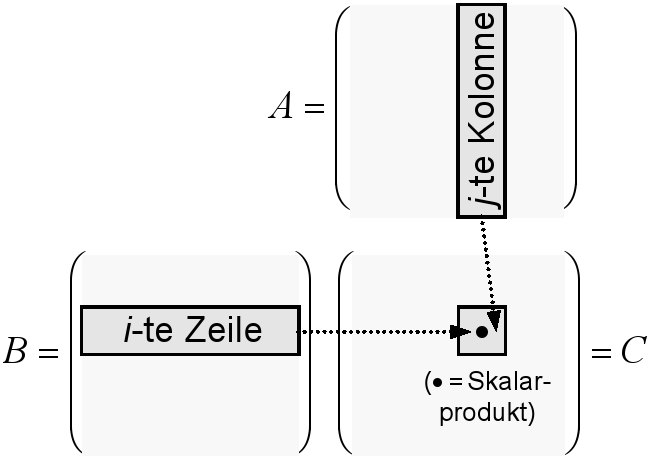
\includegraphics[width=5cm]{pics/3_Matrizenmulti}
		\end{minipage}

\subsection{Allgemeines Skalarprodukt}
	\begin{tabular}{ll}
		$\xi \bullet  \gamma = \xi^tG\gamma$ & $\xi, \gamma$ sind Vektoren\\
		$\xi' \bullet \gamma' = {\xi'}^tG'\gamma' = \xi^tT^tG'T\gamma$ & G = Symmetrische Matrix\\
		$G = T^tG'T$ & G in Standartbasis = Einheitsmatrix (E)\\
		$G' = {T^{-1}}^tGT^{-1}$ &
	\end{tabular}






















%%%%%%%%%%%%%%%%%%%%%%%%%%%%%%%%%%%%%%%%%%%%%%%%
% Zerlegungen
%%%%%%%%%%%%%%%%%%%%%%%%%%%%%%%%%%%%%%%%%%%%%%%%

\section{Zerlegungen}

\subsection{L-U-Zerlegung}
	A = LU\\
	(A gegeben)
	\begin{enumerate}
		\item Gauss (Vorwärtsreduktion)
		\item L $\rightarrow$ Pivospalten (rot und blau), U $\rightarrow$ "Rest" (grün) 
	\end{enumerate}\ 
	$\begin{array}{|cccc|}
		\hline 
		\color{red}* & * & * & *\\
		\color{blue}* & * & * & *\\
		\color{blue}* & * & * & *\\
		\color{blue}* & * & * & *\\
		\hline
	\end{array}$
	$\rightarrow$
	$\begin{array}{|cccc|}
		\hline 
		1 & * & * & *\\
		0 & \color{red}* & * & *\\
		0 & \color{blue}* & * & *\\
		0 & \color{blue}* & * & *\\
		\hline
	\end{array}$
	$\rightarrow^{...}\rightarrow$
	$\begin{array}{|cccc|}
		\hline 
		1 & * & * & *\\
		0 & 1 & * & *\\
		0 & 0 & 1 & *\\
		0 & 0 & 0 & \color{red}*\\
		\hline
	\end{array}$
	$\rightarrow$
	$\begin{array}{|cccc|}
		\hline 
		\color{green}1 & \color{green}* & \color{green}* & \color{green}*\\
		0 & \color{green}1 & \color{green}* & \color{green}*\\
		0 & 0 & \color{green}1 & \color{green}*\\
		0 & 0 & 0 & \color{green}1\\
		\hline
	\end{array}$\ \ \ \
	$L=	\left(\begin{array}{cccc}
			\color{red}* & 0 & 0 & 0\\
		 	\color{blue}* & \color{red}* & 0 & 0\\
			\color{blue}* & \color{blue}* & \color{red}* & 0\\
			\color{blue}* & \color{blue}* & \color{blue}* & \color{red}*\\
	\end{array}\right)$\ \ \ \ \ \ 
	$U=	\left(\begin{array}{cccc}
			\color{green}* & \color{green}* & \color{green}* & \color{green}*\\
		 	0 & \color{green}* & \color{green}* & \color{green}*\\
			0 & 0 & \color{green}* & \color{green}*\\
			0 & 0 & 0 & \color{green}*\\
	\end{array}\right)$\\\\\\\\
	\textbf{Beispiel:}\ \ \ \  
	$A=	\left(\begin{array}{ccc}
		-1 &\ \ 0 &\ \ 2\\
		 \ \ 1 &\ \ 3 &\ \ 3\\
		-1 &-3 &\ \ 1\\
	\end{array}\right)$\\\\\\ 
	$\begin{array}{|ccc|}
			\hline 
			\color{red}-1 & \ \ 0 & \ \ 2\\
			\color{blue}\ \ 1 & \ \ 3 & \ \ 3\\
			\color{blue}-1 & -3 & \ \ 1\\
			\hline
	\end{array}$
	$\rightarrow$
	$\begin{array}{|ccc|}
			\hline 
			\ \ 1 & \ \ 0 & -2\\
			\ \ 0 & \color{red}\ \ 3 & \ \ 5\\
			\ \ 0 & \color{blue}-3 & -1\\
			\hline
	\end{array}$
	$\rightarrow$
	$\begin{array}{|ccc|}
			\hline 
			\ \ 1 & \ \ 0 & -2\\
			\ \ 0 & \ \ 1 & \ \ \frac 5 3\\
			\ \ 0 & \ \ 0 & \color{red}\ \ 4\\
			\hline
	\end{array}$
	$\rightarrow$
	$\begin{array}{|ccc|}
			\hline 
			\color{green}\ \ 1 & \color{green}\ \ 0 & \color{green}-2\\
			\ \ 0 & \color{green}\ \ 1 & \color{green}\ \ \frac 5 3\\
			\ \ 0 & \ \ 0 & \color{green}\ \ 1\\
			\hline
	\end{array}$\ \ \ \ \	
	$L=	\left(\begin{array}{ccc}
			\color{red}-1 &\ \ 0 &\ \ 0\\
		 	\color{blue}\ \ 1 &\color{red}\ \ 3 &\ \ 0\\
			\color{blue}-1 &\color{blue} -3 &\color{red}\ \ 4\\
	\end{array}\right)$\ \ \ \ \ \ 
	$U=	\left(\begin{array}{ccc}
			\color{green}\ \ 1 &\color{green}\ \ 0 &\color{green}-2\\
		 	\ \ 0 &\color{green}\ \ 1 &\color{green}\ \ \frac 5 3\\
			\ \ 0 &\ \ 0 &\color{green}\ \ 1\\
	\end{array}\right)$\\
		
\subsection{Q-R-Zerlegung}
	A = QR\\
	(A gegeben)
	\begin{enumerate}
		\item Q $\rightarrow$ A orthonormalisieren 
		\item R $\rightarrow$ $Q^t$A 
	\end{enumerate} 
	\textbf{Beispiel:}\ \ \ \  
	$A=	\left(\begin{array}{ccc}
		\ \ 1 &\ \ 0 &\ \ 0\\
		\ \ 1 &\ \ 1 &\ \ 0\\
		\ \ 1 &\ \ 1 &\ \ 1\\
	\end{array}\right)$
	$\rightarrow^{orthonorm.}\rightarrow$
	$\left(\begin{array}{ccc}
		\ \ \frac 1 {\sqrt 3}  & -\frac 2 {\sqrt 6} &\ \ 0\\
		\ \ \frac 1 {\sqrt 3} &\ \ \frac 1 {\sqrt 6} & -\frac 1 {\sqrt 2}\\
		\ \ \frac 1 {\sqrt 3} &\ \ \frac 1 {\sqrt 6} &\ \ \frac 1 {\sqrt 2}\\
	\end{array}\right)$ = Q\\\\\\
	R = $Q^t$A = 
	$\left(\begin{array}{ccc}
			\ \ \frac 1 {\sqrt 3}  &\ \ \frac 1 {\sqrt 3} &\ \frac 1 {\sqrt 3}\\
			 -\frac 2 {\sqrt 6} &\ \ \frac 1 {\sqrt 6} &\ \frac 1 {\sqrt 6}\\
			\ \ 0 & -\frac 1 {\sqrt 2} &\ \ \frac 1 {\sqrt 2}\\
		\end{array}\right)$ * 
	$\left(\begin{array}{ccc}
		\ \ 1 &\ \ 0 &\ \ 0\\
		\ \ 1 &\ \ 1 &\ \ 0\\
		\ \ 1 &\ \ 1 &\ \ 1\\
	\end{array}\right)$ =
	$\left(\begin{array}{ccc}
		\ \ \frac 3 {\sqrt 3} &\ \ \frac 2 {\sqrt 3} &\ \ \frac 1 {\sqrt 3}\\
		\ \ 0 &\ \ \frac 2 {\sqrt 6} &\ \ \frac 1 {\sqrt 6}\\
		\ \ 0 &\ \ 0 &\ \ \frac 1 {\sqrt 2}\\
	\end{array}\right)$

\subsection{Cholesky-Zerlegung}
	A = $LL^t$\\
	(A gegeben)\\\\ 
	$A=	\left(\begin{array}{ccc}
		\ \ l_{11} &\ \ l_{21} &\ \ l_{31}\\
		\ \ l_{12} &\ \ l_{22} &\ \ l_{32}\\
		\ \ l_{13} &\ \ l_{23} &\ \ l_{33}\\	
	\end{array}\right)$ 
	= $LL^t$ = 
	$\left(\begin{array}{ccc}
		\ \ x_1 &\ \ 0 &\ \ 0\\
		\ \ x_2 &\ \ x_4 &\ \ 0\\
		\ \ x_3 &\ \ x_5 &\ \ x_6\\	
	\end{array}\right)$ *
	$\left(\begin{array}{ccc}
		\ \ x_1 &\ \ x_2 &\ \ x_3\\
		\ \ 0 &\ \ x_4 &\ \ x_5\\
		\ \ 0 &\ \ 0 &\ \ x_6\\	
	\end{array}\right)$\\\\\\ 
	(1): $x_1*x_1 + 0*0 + 0*0 = x_1^2 = l_{11}$ $\rightarrow$ $x_1$ berechnen\\ 		
	(2): $x_2*x_1 + x_4*0 + 0*0 = x_2*x_1 = l_{12}$ $\rightarrow$ $x_2$ berechnen\\ 
	(3): $x_3*x_1 + x_5*0 + x_6*0 = x_3*x_1 = l_{13}$ $\rightarrow$ $x_3$ berechnen\\
	(4): $x_2*x_2 + x_4*x_4 + 0*0 = x_2^2 + x_4^2 = l_{22}$ $\rightarrow$ $x_4$ berechnen\\
	(5): $x_3*x_2 + x_5*x_4 + x_6*0 = x_3*x_2 + x_5*x_4 = l_{23}$ $\rightarrow$ $x_5$ berechnen\\	
	(6): $x_3*x_3 + x_5*x_5 + x_6*x_6 = x_3^2 + x_5^2 + x_6^2 = l_{33}$ $\rightarrow$ $x_6$ berechnen\\	








%%%%%%%%%%%%%%%%%%%%%%%%%%%%%%%%%%%%%%%%%%%%%%%%
% Eigenwerte und Eigenvektoren
%%%%%%%%%%%%%%%%%%%%%%%%%%%%%%%%%%%%%%%%%%%%%%%%
\section{Eigenwerte und Eigenvektoren}
	Wenn eine Abbildung auf denselben Punkt fällt ($\vec{v} = \vec{v}'$), nennt man dies Eigenfixpunkt.
	Der Eigenvektor $\vec{v}$ zeigt nun in diese Richtung (als Gerade) und der Eigenwert $\lambda$ gibt den Faktor an, mit der in
	diese Richtung gezeigt wird. D.h. es gilt
	\begin{equation*}
		Av = \lambda v
	\end{equation*}

	\textbf{Def.:} Eine Matrix heisst diagonalisierbar, wenn es eine Basis aus den Eigenvektoren gibt.\\

	\textbf{Def.:} Symmetrische Matrizen sind diagonalisierbar (die Eigenwerte stehen in der Diagonalen). 
	Es gibt eine orthonormierte Eigenvektorbasis.

	\subsection{Berechnen der Eigenwerte}
		\begin{enumerate}
			\item Determintante ausrechnen
			\item Gleichung lösen (Lösungen = Eigenwerte)
		\end{enumerate}
		\begin{equation*}
			det(A - \lambda E) = 0
		\end{equation*}
		
		Beispiel:
		\begin{equation*}
			A = \left(\begin{array}{cc}
				a_1 & b_1\\
				a_2 & b_2
			\end{array}\right) \\ \Longrightarrow\\
			\left|\begin{array}{cc}
				a_1 - \lambda & b_1\\
				a_2 & b_2 - \lambda
			\end{array}\right| = 0 \\ \Longrightarrow\\
			\lambda^2 -\lambda(a_1 + b_2) + a_1b_2 - a_2b_1 = 0
		\end{equation*}
		
		\textbf{Def.:} $det(A - \lambda E)$ heisst charakteristisches Polynom $\chi_A$\\

	\subsection{Berechnen der Eigenvektoren}
		\textbf{Für jeden Eigenwert $\lambda_i$}  Gleichungssystem aufstellen und mit Gauss auflösen $\Rightarrow$ eine Zeile
		verschwindet $\Rightarrow \infty$ Lösungen $\Rightarrow$ Wert von verschwundener Zeile frei wählbar.
		\begin{equation*}
			(A - \lambda_i E)\vec{v_i} = 0
		\end{equation*}

		Beispiel:
		\begin{equation*}
			\left|\begin{array}{ccc}
				v_1 - 2v_2 & = & 0\\
				0 & = & 0
			\end{array}\right| \\
			\Rightarrow \\
			v_2 \text{ ist frei wählbar} \\
			\Rightarrow \\
			\begin{array}{c}
				v_1 = 2v_2\\
				v_2 = x
			\end{array} \\
			\Rightarrow \\
			\vec{v} = \left(\begin{array}{c}
				v_1 \\
				v_2
			\end{array}\right) = \left(\begin{array}{c}
				2v_2\\
				v_2
			\end{array}\right) = \left(\begin{array}{c}
				2x \\
				x
			\end{array}\right) = x \cdot \left(\begin{array}{c}
				2 \\
				1
			\end{array}\right)
		\end{equation*}

	\subsection{Potenzrechen von Matrizen}
		\begin{equation*}
			A^k = T^{-1}{A'}^kT = T^{-1}\left(\begin{array}{ccc}
				{\lambda_1}^k & & 0\\
				& \ddots & \\
				0 & & {\lambda_n}^k
			\end{array}\right) T
		\end{equation*}
		\begin{equation*}
			A' = \left(\begin{array}{ccc}
				{\lambda_1}^k & & 0\\
				& \ddots & \\
				0 & & {\lambda_n}^k
			\end{array}\right) 
			A' \text{ in Eigenvektoren-Basis}
		\end{equation*}
		\begin{equation*}
			T = (Ev_1, Ev_2, \ldots, Ev_n)^{-1}
		\end{equation*}

	\subsection{Rekursionsformel}
		$x_{n+3} = 4x_n - 11x_{n+1} + 6x_{n+2}$\\
		\begin{enumerate}
			\item Matrix/Vektor Schreibweise : $\left(\begin{array}{c}
					x_{n+3}\\
					x_{n+2}\\
					x_{n+1}
				\end{array}\right) = A\left(\begin{array}{c}
					x_{n+2}\\
					x_{n+1}\\
					x_n
				\end{array}\right) \qquad \qquad A = \left(\begin{array}{ccc}
					6 & -11 & 4\\
					1 & 0 & 0\\
					0 & 1 & 0
				\end{array}\right)$

			\item $\vec{u}$ ein Eigenvektor von $A$ \qquad $A^nu = \lambda^nu$ \\
				$\left(\begin{array}{c}
					x_{n+2}\\
					x_{n+1}\\
					x_n
				\end{array}\right) = 
				a_1{\lambda_1}^n\vec{u_1}+a_2{\lambda_2}^n\vec{u_2}+ a_3{\lambda_3}^n\vec{u_3} =
				a_1{\lambda_1}^n\left(\begin{array}{c}
					u_{11}\\
					u_{12}\\
					u_{13}
				\end{array}\right) + a_2{\lambda_2}^n\left(\begin{array}{c}
					u_{21}\\
					u_{22}\\
					u_{23}
				\end{array}\right) + a_3{\lambda_3}^n\left(\begin{array}{c}
					u_{31}\\
					u_{32}\\
					u_{33}
				\end{array}\right)$ \\
				$x_n = a_1{\lambda_1}^nu_{13} + a_2{\lambda_2}^nu_{23} + a_3{\lambda_3}^nu_{33}$
		\end{enumerate}



































\end{document}